%%%%%%%%%%%%%%%%%%%%%%%%%%%%%%%%%%%%%%%%%
% Short Three-Column Newsletter
% LaTeX Template
% Version 1.0 (11/9/13)
%
% Original author:
% Frits Wenneker (http://www.howtotex.com) 
% With extensive modifications by:
% Vel (vel@latextemplates.com)
% 
% This template has been downloaded from:
% http://www.LaTeXTemplates.com
%
% License:
% CC BY-NC-SA 3.0 (http://creativecommons.org/licenses/by-nc-sa/3.0/)
%
%%%%%%%%%%%%%%%%%%%%%%%%%%%%%%%%%%%%%%%%%

%----------------------------------------------------------------------------------------
%	PACKAGES AND DOCUMENT CONFIGURATIONS
%----------------------------------------------------------------------------------------

\documentclass[10pt,a4paper,ngerman,twoside]{article} % Paper type (a4paper, usletter or legal) and font size (10, 11 or 12)

%\setlength\topmargin{-80mm} % Top margin
\setlength\topmargin{-48pt} % Top margin
\setlength\headheight{0pt} % Header height
\setlength\textwidth{7.0in} % Text width
\setlength\textheight{9.5in} % Text height
\setlength\oddsidemargin{-30pt} % Left margin
\setlength\evensidemargin{-30pt} % Left margin (even pages) - only relevant with 'twoside' article option
%\setlength\inner{4cm}
%\setlenfth\outer{2cm}
%\usepackage{geometry}
%\geometry{bindingoffset=20mm}
%\setlength\bindingoffset{2cm}

\usepackage{charter} % Charter font for main content

\frenchspacing % Reduces space after periods to make text more compact for a three-column layout
\usepackage{babel}
\usepackage[utf8]{inputenc}
\usepackage{graphicx} % Required for including images
\usepackage{amssymb} % Math packages
\usepackage{amsmath} 
\usepackage{multicol} % Required for the three-column layout of the document
\usepackage{url} % Clickable links
\usepackage{enumitem} % Reduces the amount of space within and between lists with [noitemsep,nolistsep]
\usepackage{marvosym} % Required for the use of symbols
\usepackage{wrapfig} % Allows wrapping text around figures
%\usepackage[T1]{fontenc} % Use 8-bit encoding that has 256 glyphs
\usepackage{datetime} % Required for defining a custom date style
\newdateformat{mydate}{\monthname[\THEMONTH] \THEYEAR} % Set a custom date format
\usepackage[pdfpagemode=FullScreen, colorlinks=false]{hyperref} % Link colors and PDF behavior in Acrobat
\usepackage{fancyhdr} % Required to define custom headers/footers
\usepackage{hyperref} % funktioniert nicht ?
\pagestyle{fancy} % Enables the custom headers/footers for all pages following this

%-----------------------------------------------------------
% Header and footer
\lfoot{\footnotesize % Left footer containing newsletter contact information
%\begin{wrapfigure}{l}{2.0cm}
%
\includegraphics[width=2cm]{ccbysa88x31.png} 
%\end{wrapfigure}
R.I.S. Journal Ausgabe 001, Jänner 2014: \textbf{R}emix, \textbf{I}mprove, \textbf{S}hare. Das freie, creativ-commons lizensierte Journal.  \\
\Mundus\ Download und andere Formate: \href{http://spielend-programmieren.at/de:ris:start}{\texttt{spielend-programmieren.at/de:ris:start}} \quad
%\Telefon\ (000) 111-1111 \quad
\Letter\ \href{mailto:horst.jens@spielend-programmieren.at}{horst.jens@spielend-programmieren.at}
}

\cfoot{} % Empty center footer

\rfoot{\footnotesize ~\\ Seite \thepage} % Right footer - page counter

\renewcommand{\headrulewidth}{0.0pt} % No horizontal rule for the header
\renewcommand{\footrulewidth}{0.4pt} % Horizontal rule separating the footer from the document
%-----------------------------------------------------------

%-----------------------------------------------------------
% Define separators
\newcommand{\HorRule}[1]{\noindent\rule{\linewidth}{#1}} % Creates a horizontal rule
\newcommand{\SepRule}{\noindent	% Creates a shorter separator rule
\begin{center}
\rule{250pt}{1pt} % Page width and rule width
\end{center}
}
\newcommand{\Trenner}{\noindent
\begin{center}
\rule{100pt}{1pt}
\end{center}
}
%-----------------------------------------------------------

%-----------------------------------------------------------
% Define title and article styles
\newcommand{\NewsletterName}[1]{ % Newsletter title
\begin{center}
\Huge \usefont{T1}{fvs}{b}{n} % Use the Bera Sans Bold font
#1
\end{center}	
\par \normalsize \normalfont}

\newcommand{\JournalIssue}[1]{ % Date and issue number at the top of the newsletter
%\hfill \textsc{\mydate \today, No #1} % Right-aligned date and issue number
\hfill \textsc{Jänner 2014, Ausgabe 001}
\par \normalsize \normalfont}

\newcommand{\NewsItem}[1]{ % News item title
\usefont{T1}{fvs}{n}{n} % Use the Bera Sans Normal font
\vspace{24pt}\large #1\vspace{3pt} % Print the title with space around it in a larger font size
\par \normalsize \normalfont}

\newcommand{\NewsAuthor}[1]{ % Author name under the item title
\hfill von \textsc{#1} \vspace{20pt} % Right-aligned author name in small caps with space after it
\par \normalfont}		

%----------------------------------------------------------------------------------------
%	TITLE
%----------------------------------------------------------------------------------------

\begin{document}

\JournalIssue{1} % Issue number
\NewsletterName{R.I.S. Journal} % Newsletter title
%\begin{center}
%\textbf{R}emix \textbf{I}mprove \textbf{S}hare - das freie Journal für Open Source Education
%\end{center}
\noindent\HorRule{3pt} \\[-0.75\baselineskip] % Thick horizontal rule
\HorRule{1pt} % Thin horizontal rule



%\setlength{\columnsep}{16pt} % Uncomment to manually change the white space between columns
%\begin{multicols}{3} % Begin the three-column layout

%----------------------------------------------------------------------------------------
%	OTHER NEWS
%----------------------------------------------------------------------------------------
%-----------------------------------------------------------
%
%-----------------------------------------------------------
%RIS-Journal Titel (Titelgrafik hier einfügen)
\begin{multicols}{2}
\NewsItem{}
\section*{The Powder Toy Tutorial}
\label{powdertoytutorial}
\NewsAuthor{Sebastian Krähsmaier}

\textbf{Sebastian Krähsmaier (12 J) lernt gerade besucht die Programmiersprache Python bei \href{http://spielend-programmieren.at}{\textit{spielend-programmieren [1]}} und erforscht mittels \textit{The Powder Toy [2]} physikalische Zusammenhänge. In diesem Tutorial versucht er die Aufgabe zu lösen, Wasser von einem Topf links in einen Topf rechts zu befördern.}

\begin{center}
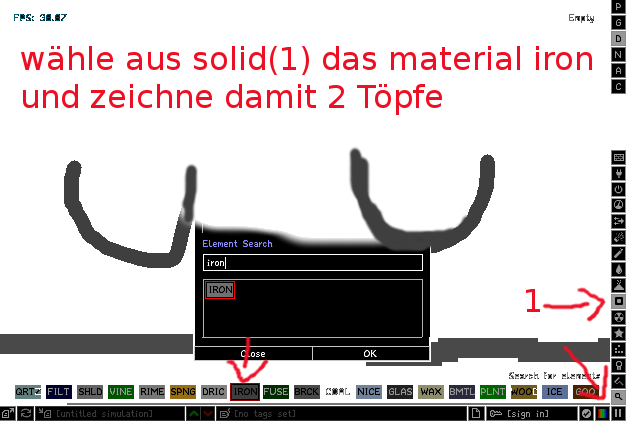
\includegraphics[width=\linewidth]{powdertoytutorial/powdertoytutorial1.png}
\end{center}

\begin{center}
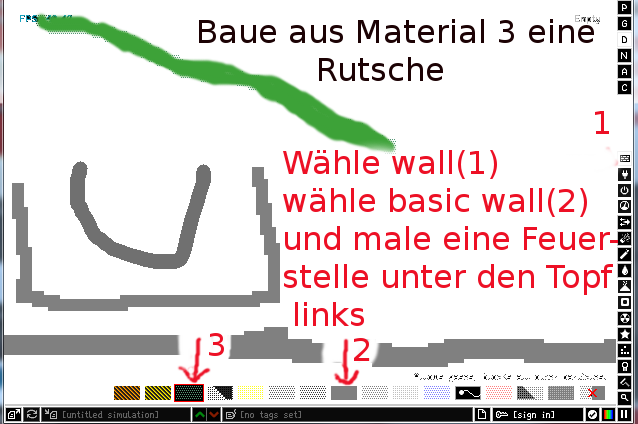
\includegraphics[width=\linewidth]{powdertoytutorial/powdertoytutorial2.png}
\end{center}

\begin{center}
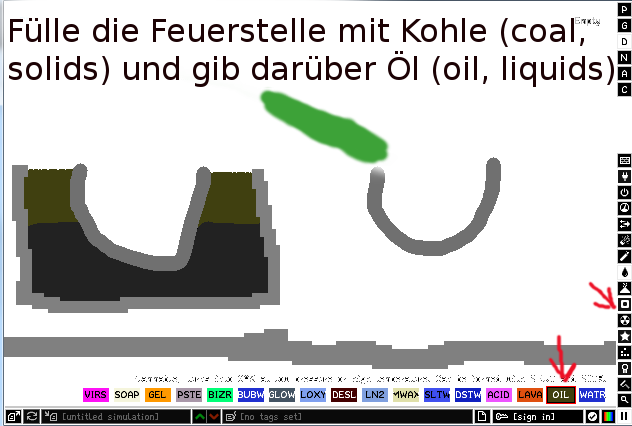
\includegraphics[width=\linewidth]{powdertoytutorial/powdertoytutorial3.png}
\end{center}

\begin{center}
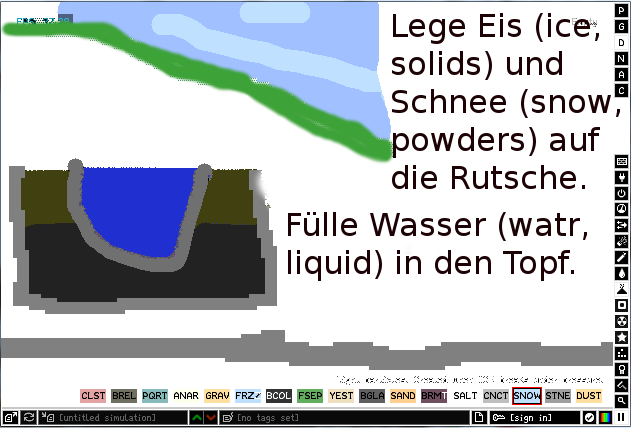
\includegraphics[width=\linewidth]{powdertoytutorial/powdertoytutorial4.png}
\end{center}

\begin{center}
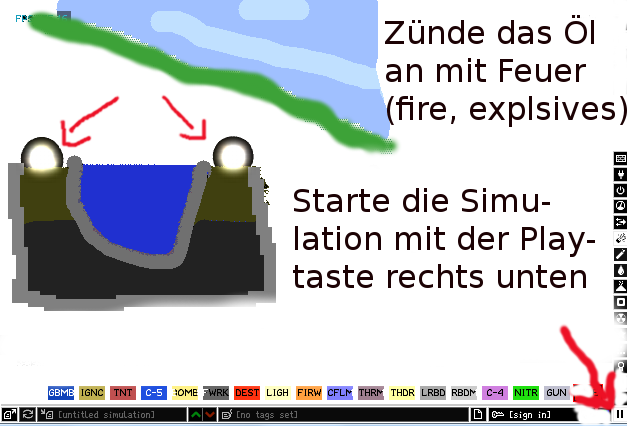
\includegraphics[width=\linewidth]{powdertoytutorial/powdertoytutorial5.png}
\end{center}

Erklärung: Die Flammen sollten das Öl anzünden und anschließend die Kohlen unter dem Metalltopf links. Da Metall wärmeleitend ist steigt aus dem Topf Wasserdampf auf. Die Rutsche über dem Topf ist dampfdurchlässig, der Dampf schmilzt den Schnee und das Eis. Da die Rutsche Flüssigkeiten abweist und nach rechts geneigt ist rinnt das Schmelzwasser in den Topf rechts. Hat man alles richtig gemacht dann verdampft das Wasser im linken Topf komplett und es sammelt sich Wasser im rechten Topf.

\subsection*{Lizenz, Quellen:}
\begin{wrapfigure}{l}{2.0cm}

\includegraphics[width=2cm]{powdertoytutorial/ccbysa88x31.png}
\end{wrapfigure}
Dieses Material steht unter der Creative-Commons-Lizenz Namensnennung - Weitergabe unter gleichen Bedingungen 4.0 International. Um eine Kopie dieser Lizenz zu sehen, besuchen Sie \url{http://creativecommons.org/licenses/by-sa/4.0/deed.de}.

\subsection*{Download, Feedback:}
\footnotesize{
Ordner \texttt{powdertoytutorial} \Mundus\ \href{http://spielend-programmieren.at/risjournal/001}{spielend-programmieren.at/risjournal/001}\\
Startseite: \href{http://spielend-programmieren.at/de:ris:001}{spielend-programmieren.at/de:ris:001}\\ 
\Letter\:  horst.jens@spielend-programmieren.at \\}
\normalsize{}

\textbf{Quellen:} \\
{[}1{]} \href{http://spielend-programmieren.at}{spielend-programmieren.at} \\
{[}2{]} \href{http://powdertoy.co.uk/}{powdertoy.co.uk/} \\
\end{multicols}
%\SepRule
%-----------------------------------------------------------
\end{document}
